%----------------------------------------------------------------------------------------
%   PHẦN 2: CƠ SỞ LÝ THUYẾT
%----------------------------------------------------------------------------------------
\section{Cơ sở lý thuyết}

%--- YOLO ---
\begin{frame}{Tổng quan về Phát hiện đối tượng}
    \begin{itemize}
        \item \textbf{Định nghĩa:} Xác định vị trí và phân loại các đối tượng trong ảnh/video
        \item \textbf{Đầu ra:} Tập hợp bounding box $B = \{b_1, b_2, \dots, b_N\}$
        $$ b_i = (x_i, y_i, w_i, h_i, c_i, p_i) $$
        \begin{itemize}
            \item $(x_i, y_i)$: Tọa độ tâm
            \item $(w_i, h_i)$: Kích thước khung bao
            \item $c_i$: Nhãn lớp (xe máy, ô tô, ...)
            \item $p_i$: Độ tin cậy (confidence)
        \end{itemize}
        \item \textbf{Thách thức:} Biến thiên tỷ lệ, bị che khuất, biến dạng hình học
    \end{itemize}
\end{frame}

\begin{frame}{Lựa chọn mô hình: YOLOv8}
    \textbf{Lý do lựa chọn YOLOv8 cho bài toán giao thông:}
    \begin{itemize}
        \item \textbf{Anchor-free:} Loại bỏ anchor box thủ công, linh hoạt với các đối tượng có tỷ lệ biến thiên lớn
        \item \textbf{Module C2f:} Cải thiện luồng gradient, trích xuất đặc trưng phong phú
        \item \textbf{Task Aligned Assigner:} Cân bằng giữa điểm phân loại và độ chính xác định vị
        \item \textbf{Hiệu năng:} Cân bằng tốt giữa tốc độ (Real-time) và độ chính xác (mAP)
    \end{itemize}

    \vspace{0.5em}
    \begin{alertblock}{YOLOv8n (Nano)}
    Phiên bản nhẹ nhất (3.2M params), phù hợp cho ứng dụng real-time trên GPU phổ thông
    \end{alertblock}
\end{frame}

\begin{frame}{Kiến trúc YOLOv8}
    \begin{figure}
        \centering
        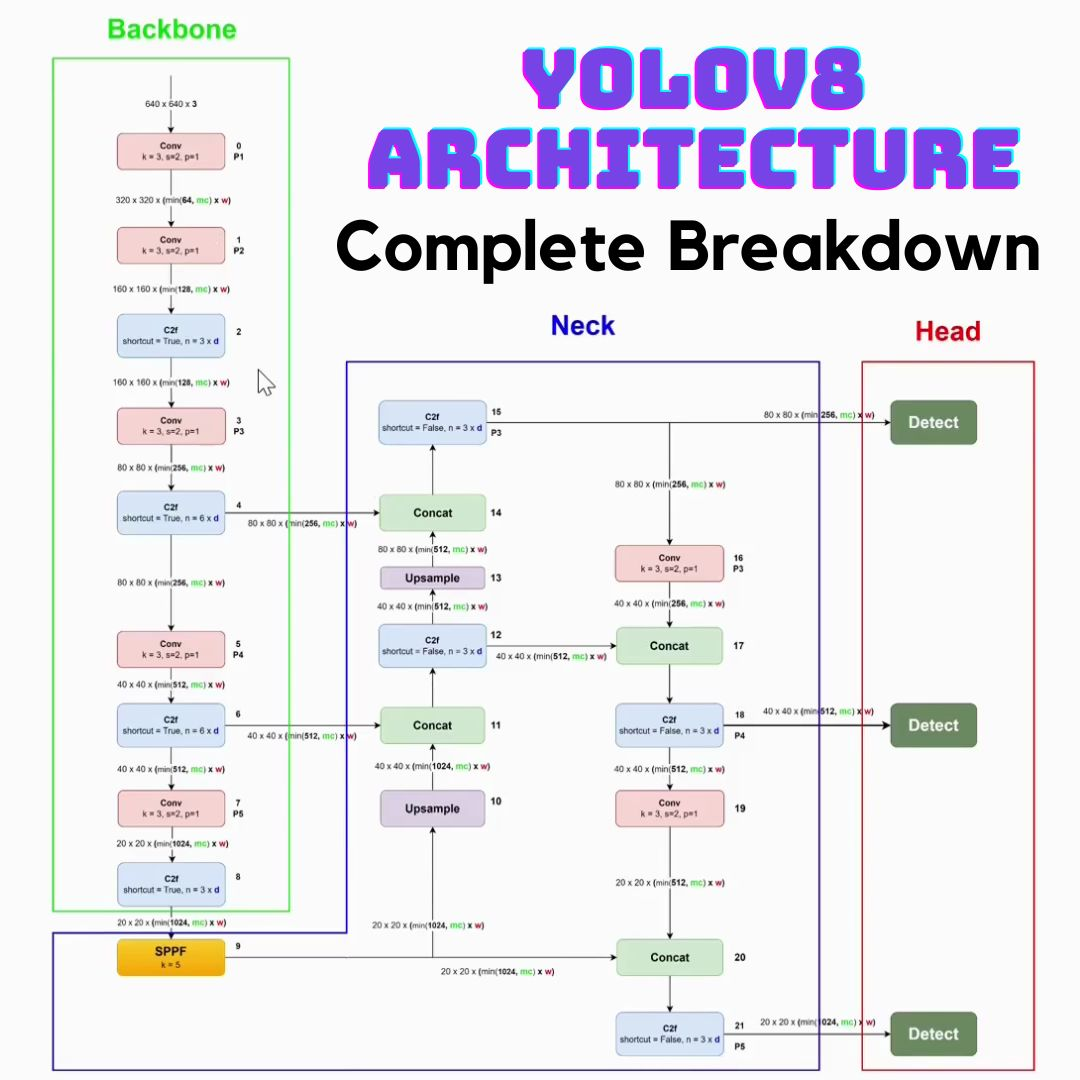
\includegraphics[width=0.55\linewidth]{Figures/1698478493766.jpg}
        \caption{Kiến trúc tổng thể YOLOv8}
    \end{figure}

\end{frame}

\begin{frame}{Hàm mất mát YOLOv8}
    Tối thiểu hóa hàm mất mát tổng hợp:
    $$ L_{total} = \lambda_{box} L_{box} + \lambda_{cls} L_{cls} + \lambda_{dfl} L_{dfl} $$

    \begin{block}{Các thành phần chính}
    \begin{itemize}
        \item \textbf{CIoU Loss ($L_{box}$):} Định vị bounding box
        $$ \mathcal{L}_{CIoU} = 1 - IoU + \frac{\rho^2(\mathbf{b}, \mathbf{b}^{gt})}{c^2} + \alpha v $$
        \item \textbf{Distribution Focal Loss (DFL):} Tối ưu cho box có biên mờ
        \item \textbf{Varifocal Loss ($L_{cls}$):} Cân bằng mẫu khó/dễ
    \end{itemize}
    \end{block}
\end{frame}

%--- BYTETRACK ---
\begin{frame}{Theo dõi đa đối tượng (MOT)}
    \textbf{Mục tiêu:} Gán ID duy nhất cho mỗi đối tượng qua các khung hình liên tiếp

    \begin{block}{Phương pháp: Tracking-by-Detection}
    \begin{itemize}
        \item \textbf{Bộ lọc Kalman:} Ước lượng trạng thái (vị trí, vận tốc) để dự đoán vị trí tiếp theo
        \item \textbf{Thuật toán Hungarian:} Ghép cặp tối ưu giữa \textit{Dự đoán Kalman} và \textit{Phát hiện YOLO}
    \end{itemize}
    \end{block}

    \begin{figure}
        \centering
        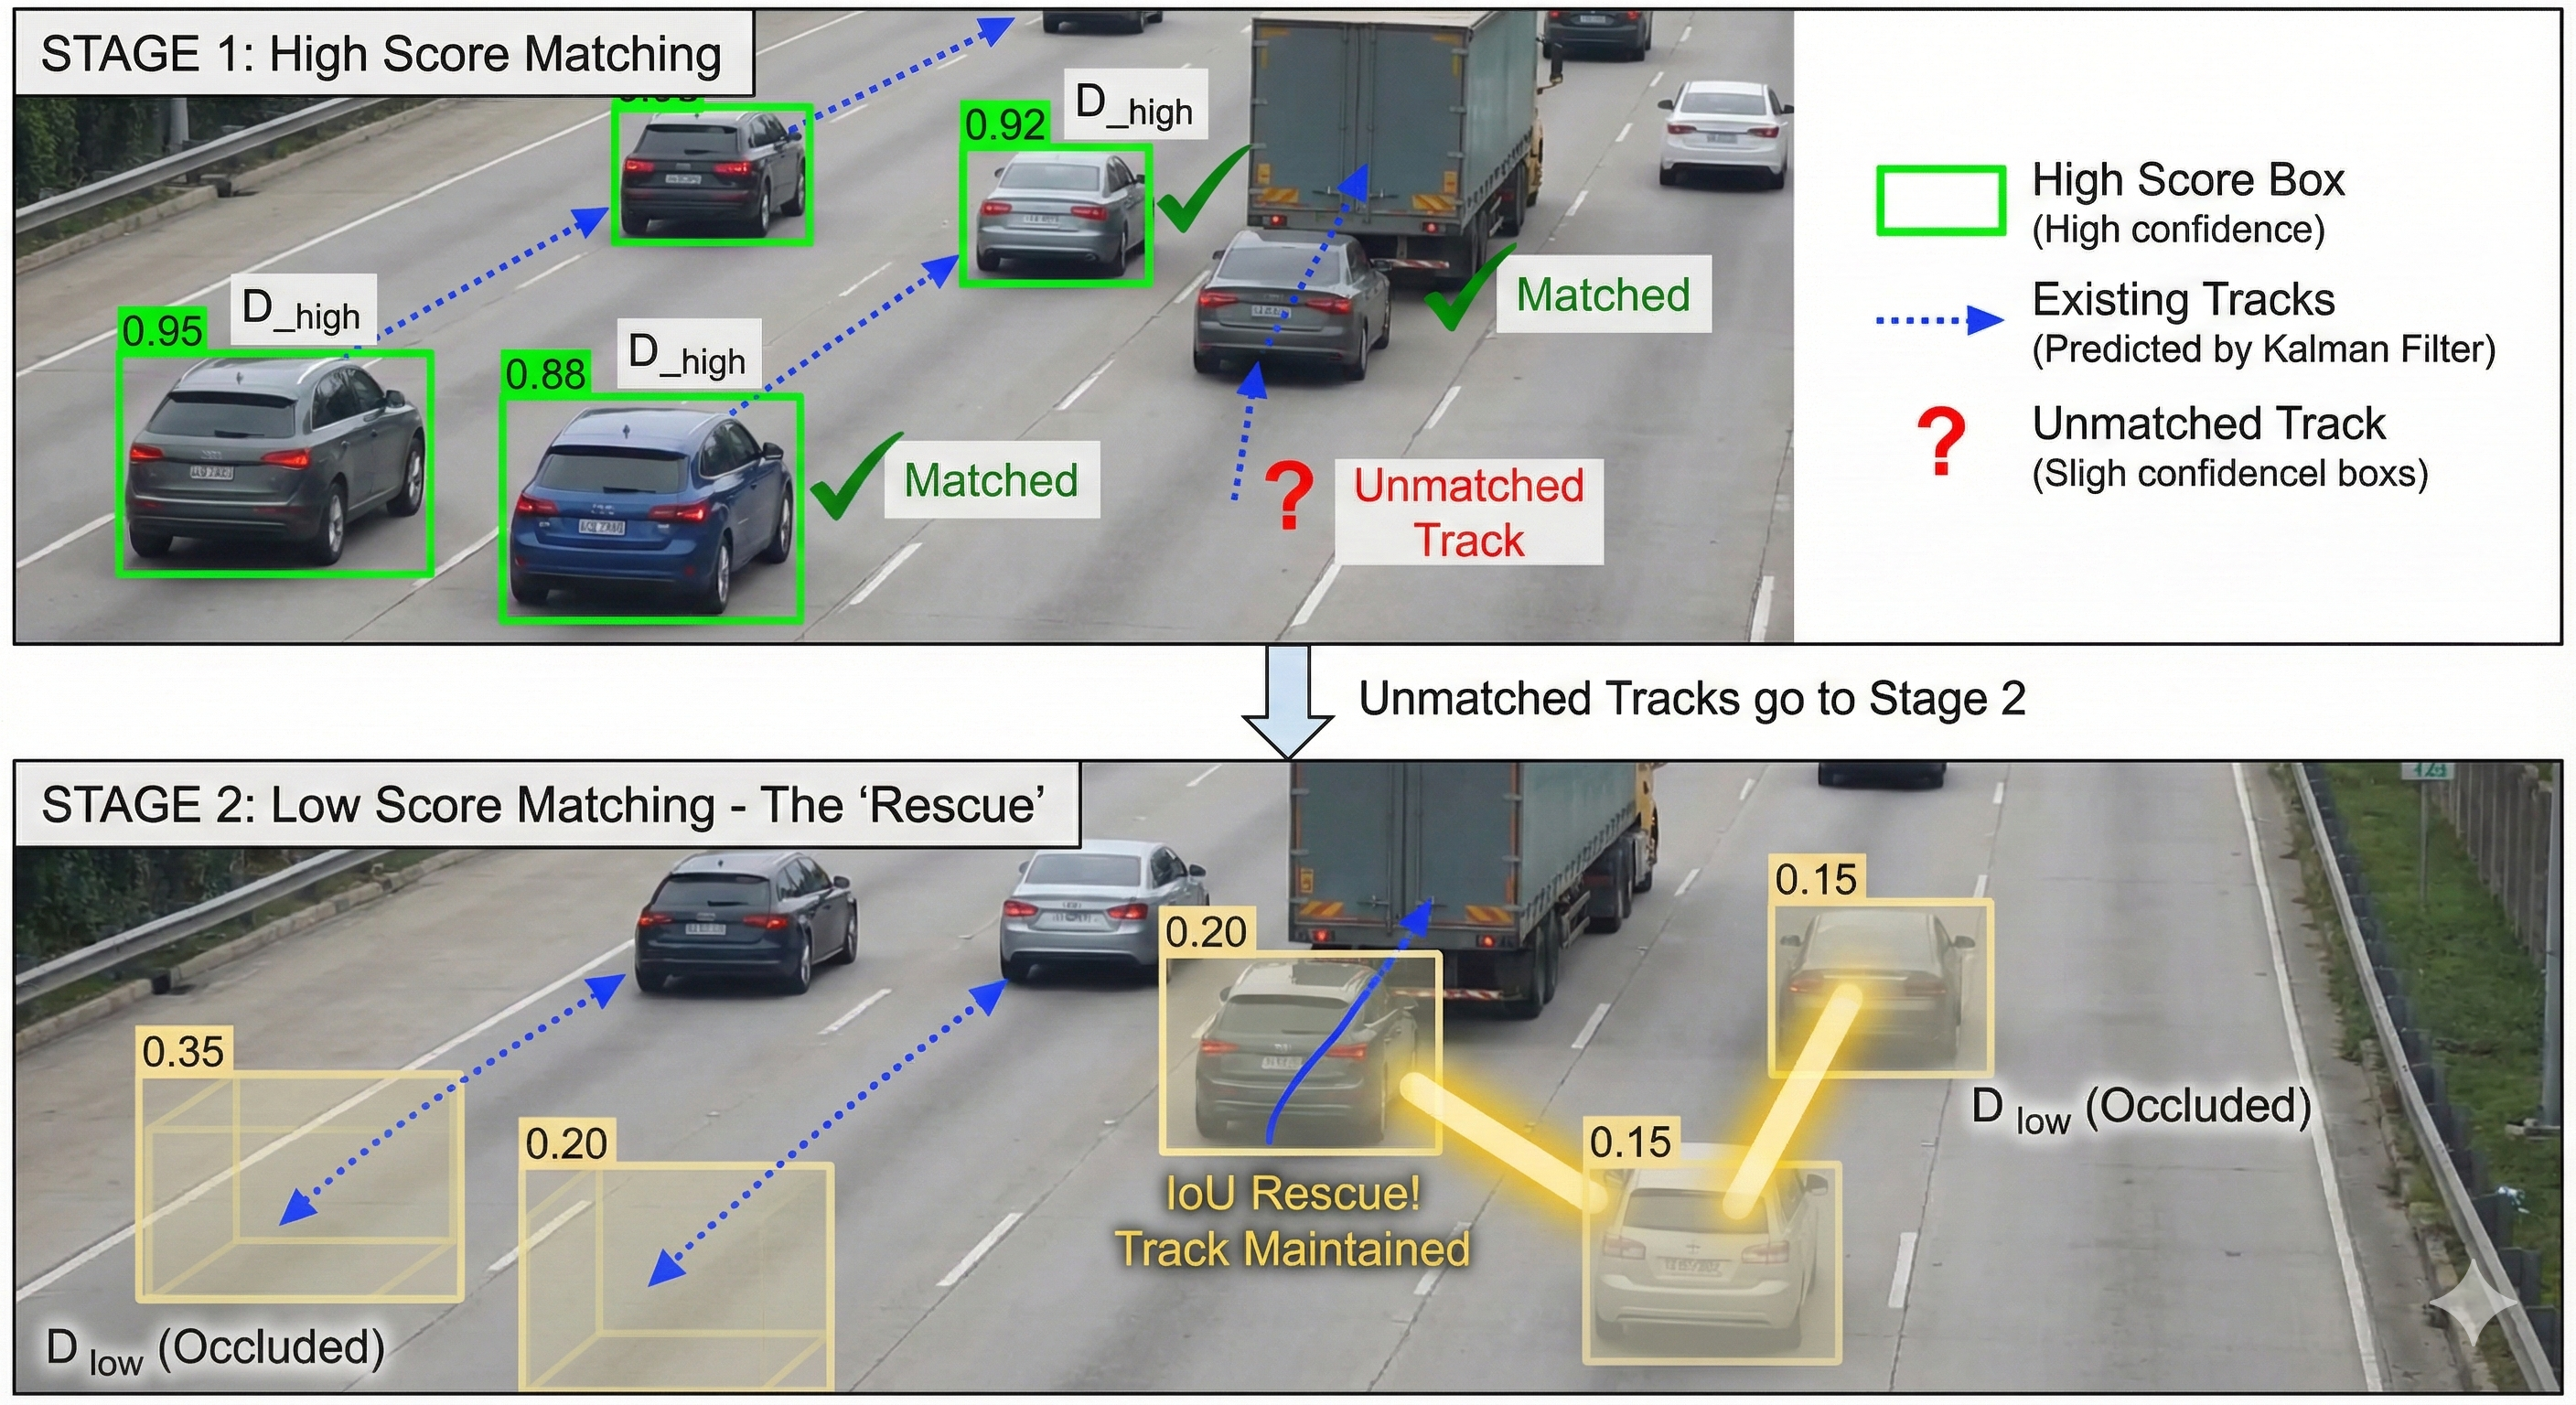
\includegraphics[width=0.5\linewidth]{Figures/bytetrack.png}

    \end{figure}
\end{frame}

\begin{frame}{Thuật toán ByteTrack}
    \textbf{Ý tưởng:} "Tận dụng mọi detection, kể cả độ tin cậy thấp"

    \begin{block}{Quy trình 2 giai đoạn}
    \begin{enumerate}
        \item \textbf{High Score Matching:}
        \begin{itemize}
            \item Ghép detection chất lượng cao ($conf > \tau_{high}$) với Track hiện có
            \item Sử dụng IoU làm trọng số
        \end{itemize}
        \item \textbf{Low Score Matching:}
        \begin{itemize}
            \item Track chưa ghép sẽ tìm trong detection chất lượng thấp ($conf > \tau_{low}$)
            \item "Cứu" lại xe bị che khuất hoặc mờ
        \end{itemize}
    \end{enumerate}
    \end{block}

    \textbf{Ưu điểm:} Tốc độ cao (không cần trích xuất đặc trưng ngoại hình)
\end{frame}

%--- NHẬN DIỆN ĐÈN GIAO THÔNG ---
\begin{frame}{Nhận diện đèn giao thông (HSV)}
    \begin{block}{Chuyển đổi RGB $\rightarrow$ HSV}
    Tách biệt thông tin màu sắc và độ sáng
    \end{block}

    \textbf{Ngưỡng màu cho từng trạng thái đèn:}
    \begin{itemize}
        \item \textbf{Đỏ (Red):} $Hue \in [0, 10] \cup [160, 180]$ (red-wrap effect)
        \item \textbf{Vàng (Yellow):} $Hue \in [15, 35]$
        \item \textbf{Xanh (Green):} $Hue \in [40, 90]$
    \end{itemize}

    \begin{block}{Cơ chế Voting}
    Tính tỷ lệ pixel cho từng mặt nạ màu $\rightarrow$ Xác định trạng thái trội
    \end{block}

    \textit{Hỗ trợ 4 loại đèn: Tròn, Rẽ trái, Rẽ phải, Đi thẳng}
\end{frame}

%--- LOGIC VI PHẠM ---
\begin{frame}{Thuật toán phát hiện Vượt đèn đỏ}
    \begin{block}{Quy trình quyết định (Decision Flow)}
    Khi sự kiện \textit{Stopline Crossing} xảy ra:
    \begin{enumerate}
        \item \textbf{Kiểm tra Quyền đi (Green Priority):}
        \begin{itemize}
            \item Có đèn xanh mũi tên trùng hướng xe? $\rightarrow$ \textcolor{green}{\textbf{HỢP LỆ}}
        \end{itemize}

        \item \textbf{Kiểm tra Cấm (Red Constraint):}
        \begin{itemize}
            \item Đèn đỏ tròn hoạt động? HOẶC Đèn đỏ mũi tên trùng hướng xe?
            \item $\rightarrow$ Nếu Đúng: \textcolor{red}{\textbf{VI PHẠM}}
        \end{itemize}

        \item \textbf{Xác nhận:} Loại trừ ngoại lệ (xe ưu tiên)
    \end{enumerate}
    \end{block}
\end{frame}

\begin{frame}{Thuật toán phát hiện Đi sai làn}
    \textbf{Cấu hình Lane Manager:}
    \begin{itemize}
        \item Mỗi làn là một \textit{Polygon} + danh sách \texttt{allowed\_classes}
        \item Hỗ trợ làn đè (overlapping lanes)
    \end{itemize}

    \begin{block}{Quy trình kiểm tra}
    \begin{enumerate}
        \item Tính tọa độ tâm $(C_x, C_y)$ của xe từ Bounding Box
        \item \textbf{Point-in-Polygon Test:} Xác định xe thuộc làn $L_i$ nào
        \item \textbf{Class Verification:}
        $$ \text{Violation} = (C \in L_i) \land (Class_v \notin L_i.allowed) $$
    \end{enumerate}
    \end{block}

    \textit{Sử dụng Ray Casting Algorithm cho Point-in-Polygon}
\end{frame}

%============================================================
% PHẦN MỚI: LÝ THUYẾT ALPR VÀ OCR
%============================================================
\begin{frame}{Tổng quan ALPR (Nhận diện biển số)}
    \textbf{ALPR = Automatic License Plate Recognition}

    \begin{block}{Pipeline tổng quát}
    \centering
    \begin{tikzpicture}[
        scale=0.8, transform shape,
        node distance=0.3cm and 0.4cm,
        box/.style={rectangle, draw, rounded corners, minimum width=1.5cm, minimum height=0.5cm, align=center, font=\tiny},
        arrow/.style={->, thick, >=stealth}
    ]
        \node[box, fill=blue!20] (input) {Ảnh\\đầu vào};
        \node[box, fill=orange!20, right=of input] (detect) {Plate\\Detection};
        \node[box, fill=yellow!20, right=of detect] (preprocess) {Tiền xử lý\\(CLAHE)};
        \node[box, fill=green!20, right=of preprocess] (ocr) {OCR};
        \node[box, fill=purple!20, right=of ocr] (output) {Biển số};

        \draw[arrow] (input) -- (detect);
        \draw[arrow] (detect) -- (preprocess);
        \draw[arrow] (preprocess) -- (ocr);
        \draw[arrow] (ocr) -- (output);
    \end{tikzpicture}
    \end{block}

    \textbf{Thách thức nhận diện biển số Việt Nam:}
    \begin{itemize}
        \item Đa dạng định dạng: 1 dòng, 2 dòng
        \item Điều kiện thực tế: Bẩn, mờ, nghiêng
        \item Ánh sáng: Phản chiếu, bóng đổ
    \end{itemize}
\end{frame}

\begin{frame}{Biển số xe Việt Nam}
    \begin{table}
        \centering
        \small
        \begin{tabular}{|c|l|l|}
            \hline
            \textbf{Loại} & \textbf{Định dạng} & \textbf{Ví dụ} \\
            \hline
            Xe ô tô (1 dòng) & XX-Y XXXXX & 30G-07784 \\
            \hline
            Xe ô tô (2 dòng) & XX-Y / XXXXX & 30G / 07784 \\
            \hline
            Xe máy & XX-YZ / XXX.XX & 29-H1 / 234.56 \\
            \hline
        \end{tabular}
    \end{table}

    \textbf{Cấu trúc:}
    \begin{itemize}
        \item \textbf{2 số đầu:} Mã tỉnh (30 = Hà Nội, 51 = TP.HCM)
        \item \textbf{1 chữ cái:} Seri (A-Z, trừ I, O, Q)
        \item \textbf{5 số cuối:} Số thứ tự đăng ký
    \end{itemize}
\end{frame}

%--- PADDLEOCR ---
\begin{frame}{PaddleOCR - Kiến trúc CRNN}
    \textbf{CRNN = Convolutional Recurrent Neural Network}

    \begin{block}{3 thành phần chính}
    \begin{enumerate}
        \item \textbf{CNN Backbone:} Trích xuất đặc trưng không gian từ ảnh
        \begin{itemize}
            \item Sử dụng MobileNet/ResNet biến thể
        \end{itemize}
        \item \textbf{Sequence Modeling (Bi-LSTM):}
        \begin{itemize}
            \item Mô hình hóa quan hệ tuần tự giữa các ký tự
            \item Bidirectional: capture thông tin cả 2 hướng
        \end{itemize}
        \item \textbf{CTC Decoder:} Giải mã chuỗi ký tự cuối cùng
    \end{enumerate}
    \end{block}

    \centering
    \small
    Ảnh biển số $\rightarrow$ CNN $\rightarrow$ Bi-LSTM $\rightarrow$ CTC $\rightarrow$ ``30G07784''
\end{frame}

\begin{frame}{CTC Loss (Connectionist Temporal Classification)}
    \textbf{Đặc điểm:} Huấn luyện không cần alignment giữa input và output

    \begin{block}{Công thức}
    Xác suất của chuỗi output $\mathbf{l}$:
    $$ P(\mathbf{l} | \mathbf{x}) = \sum_{\pi \in \mathcal{B}^{-1}(\mathbf{l})} P(\pi | \mathbf{x}) $$

    CTC Loss = Negative log-likelihood:
    $$ \mathcal{L}_{CTC} = -\log P(\mathbf{l} | \mathbf{x}) $$
    \end{block}

    \textbf{Ví dụ:} Chuỗi mục tiêu ``AB''
    \begin{itemize}
        \item ``A-A-B-B'' $\rightarrow$ ``AB'' (loại bỏ ký tự lặp)
        \item ``A--B-'' $\rightarrow$ ``AB'' (loại bỏ blank `-')
    \end{itemize}
\end{frame}

%--- TIỀN XỬ LÝ ---
\begin{frame}{CLAHE - Cân bằng histogram thích ứng}
    \textbf{CLAHE = Contrast Limited Adaptive Histogram Equalization}

    \begin{block}{Nguyên lý hoạt động}
    \begin{enumerate}
        \item \textbf{Chia tile:} Chia ảnh thành các tile nhỏ (8×8 pixels)
        \item \textbf{HE cục bộ:} Histogram Equalization trên từng tile
        \item \textbf{Clip Limit:} Giới hạn độ tương phản (tránh khuếch đại noise)
        $$ \beta = \frac{M \times N}{L} \times \text{clipLimit} $$
        \item \textbf{Bilinear Interpolation:} Ghép các tile mượt mà
    \end{enumerate}
    \end{block}

    \textbf{Cấu hình:} \texttt{clipLimit=2.0}, \texttt{tileGridSize=(8,8)}
\end{frame}

\begin{frame}{Sharpening - Làm sắc nét}
    \textbf{Mục đích:} Tăng cường cạnh ký tự trước khi đưa vào OCR

    \begin{block}{Kernel Sharpening}
    $$ K_{sharpen} = \begin{bmatrix} 0 & -1 & 0 \\ -1 & 5 & -1 \\ 0 & -1 & 0 \end{bmatrix} $$
    \end{block}

    \textbf{Công thức pixel mới:}
    $$ I'(x,y) = 5 \cdot I(x,y) - [I(x-1,y) + I(x+1,y) + I(x,y-1) + I(x,y+1)] $$

    \textit{Tăng cường sự khác biệt giữa pixel và các pixel xung quanh \\  $\rightarrow$ Cạnh sắc nét hơn}
\end{frame}

%--- VALIDATION & RETRY ---
\begin{frame}{Character Correction - Hiệu chỉnh ký tự}
    \textbf{Vấn đề:} OCR có thể nhầm lẫn ký tự tương tự

    \begin{table}
        \centering
        \small
        \begin{tabular}{|c|c|l|}
            \hline
            \textbf{Sai} & \textbf{Đúng} & \textbf{Điều kiện} \\
            \hline
            0 (số) & O (chữ) & Vị trí chữ cái (index 2) \\
            \hline
            O (chữ) & 0 (số) & Vị trí chữ số \\
            \hline
            1 (số) & I (chữ) & Vị trí chữ cái \\
            \hline
            8 (số) & B (chữ) & Vị trí chữ cái \\
            \hline
        \end{tabular}
    \end{table}

    \textbf{Logic hiệu chỉnh theo định dạng VN:}
    \begin{itemize}
        \item Vị trí 0-1: Bắt buộc chữ số (mã tỉnh)
        \item Vị trí 2: Bắt buộc chữ cái (seri)
        \item Vị trí 3+: Bắt buộc chữ số
    \end{itemize}
\end{frame}

\begin{frame}{Format Validation \& Retry Mechanism}
    \textbf{Vấn đề:} OCR có thể cho kết quả khác nhau giữa các frame
    \begin{itemize}
        \item Biển số bị rung, blur khi xe di chuyển
        \item Ánh sáng thay đổi, góc nhìn thay đổi
    \end{itemize}

    \begin{block}{Giải pháp: Format Validation}
    Validate theo định dạng biển số Việt Nam:
    \begin{itemize}
        \item \textbf{Xe máy:} \texttt{[0-9]\{2\}[A-Z][A-Z0-9][0-9]\{4,5\}} (8-9 ký tự)
        \item \textbf{Ô tô:} \texttt{[0-9]\{2\}[A-Z][0-9]\{4,5\}} (7-8 ký tự)
    \end{itemize}
    \end{block}

    \textbf{Retry Mechanism:}
    \begin{itemize}
        \item Sai format $\rightarrow$ không lưu, thử lại frame sau
        \item Đã có kết quả valid $\rightarrow$ dừng OCR (tiết kiệm tài nguyên)
    \end{itemize}
\end{frame}

%--- HƯỚNG DI CHUYỂN ---
\begin{frame}{Xác định hướng di chuyển}
    \textbf{Direction Fusion - Kết hợp 2 nguồn:}

    \begin{columns}
        \column{0.5\textwidth}
        \begin{block}{Nguồn 1: Trajectory}
        \begin{itemize}
            \item Tính vector chuyển động từ lịch sử vị trí
            \item So sánh với Reference Vector
            \item Khử nghiêng camera
        \end{itemize}
        \end{block}

        \column{0.5\textwidth}
        \begin{block}{Nguồn 2: ROI-based}
        \begin{itemize}
            \item Xác định hướng dựa trên vùng xe đang đi qua
            \item Cấu hình sẵn cho từng làn
        \end{itemize}
        \end{block}
    \end{columns}

    \vspace{0.5em}
    \textbf{Góc lệch:}
    $$ \alpha = \operatorname{atan2}(\vec{v} \times \vec{r}, \ \vec{v} \cdot \vec{r}) $$

    Trong đó $\vec{v}$: vector chuyển động xe, $\vec{r}$: vector tham chiếu đường
\end{frame}
